\documentclass[tikz]{standalone}
\usetikzlibrary{arrows, positioning}
\usetikzlibrary {arrows.meta}
\usepackage{xcolor}
\definecolor{allcolor}{RGB}{148,182,233}
\newcommand*{\equal}{=}
\begin{document}
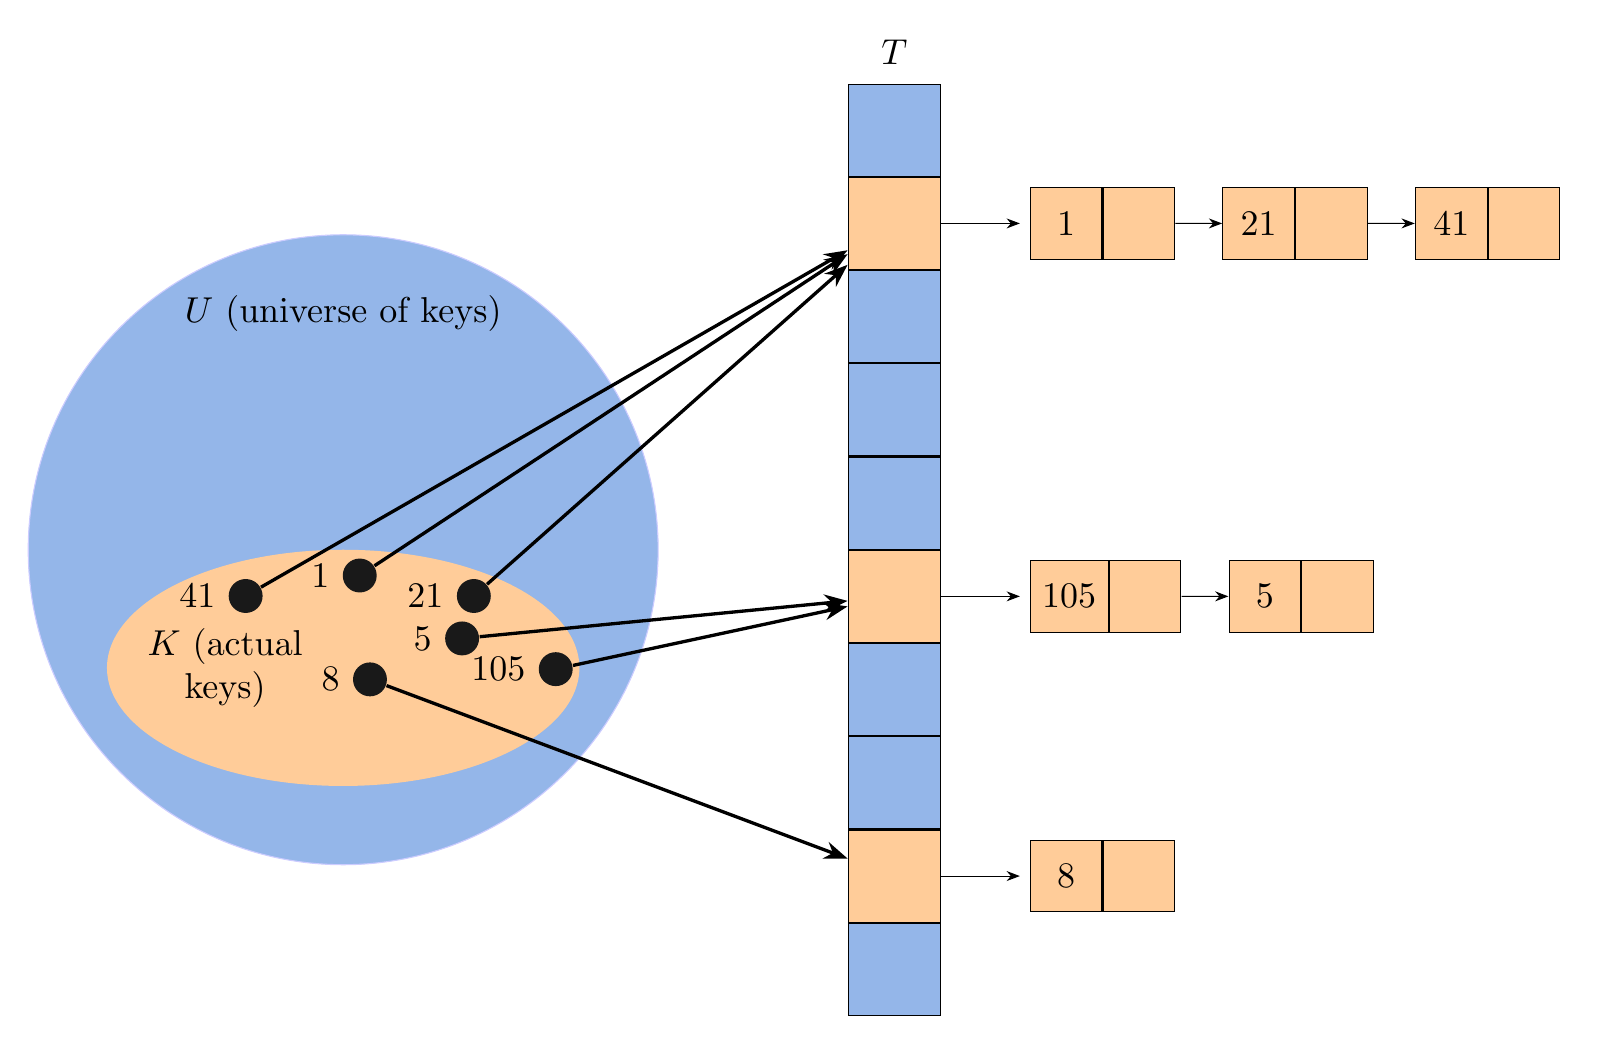
\begin{tikzpicture}[every node/.style={scale=1.3}, dot/.style={minimum size=0.1mm, circle, fill=black!90}, slot/.style={minimum size=0.9cm, rectangle}, noslot/.style={slot, fill=allcolor},
    yesslot/.style={slot, fill=orange!40}, data/.style={minimum size=0.7cm, fill=orange!40}, >=Stealth]
    \tikzstyle{textbf} = [text width=5cm,text centered]

    \filldraw[color=blue!20, fill=allcolor](0,0) circle (4);
    \node[textbf] (universe) at (0, 3) {$U$ (universe of keys)};

    \fill[orange!40] (0, -1.5) ellipse (3 and 1.5);
    \node[textbf, text width=2cm] (keys) at (-1.5, -1.5) {$K$ (actual keys)};

    \node[dot, label=left:$1$] [above right=of keys, xshift=-0.7cm, yshift=-0.5cm] (k1){};
    \node[dot, label=left:$21$] [right=of k1, yshift=-0.2cm] (k16) {};
    \node[dot, label=left:$41$] [left=of k1, yshift=-0.2cm] (k6) {};
    \node[dot, label=left:$5$,xshift=1cm, yshift=0.5cm] [below=of k1] (k5){};
    \node[dot, label=left:$105$,xshift=1cm, xshift=-1.2cm, yshift=-0.3cm] [right=of k5] (k105){}; 
    \node[dot, label=left:$8$] [below=of k1, yshift=0.1cm, xshift=0.1cm] (k8){};
    \matrix [column sep=1cm,nodes=draw] (table) at (7, 0)
    {
      \node[noslot] {}; \\ 
      \node[yesslot] (s1) {}; \\
      \node[noslot]  {}; \\
      \node[noslot]  {}; \\
      \node[noslot] {}; \\
      \node[yesslot] (s5) {}; \\
      \node[noslot] {}; \\
      \node[noslot] {}; \\
      \node[yesslot] (s8) {}; \\
      \node[noslot] {}; \\
    };

    \node[textbf, above=of table,yshift=-0.8cm]{$T$};
    \draw[->, very thick]  (k1) to (s1);
    \draw[->, very thick]  (k16) to (s1);
    \draw[->, very thick]  (k6) to (s1);
    \draw[->, very thick]  (k5) to (s5);
    \draw[->, very thick]  (k105) to (s5);
    \draw[->, very thick]  (k8) to (s8);

    \matrix [nodes=draw, right=of s1] (data1)
    {
      \node[data] {1}; & \node[data] (vv1) {}; \\
    };

    \draw[->] (s1) to (data1);

    \matrix [nodes=draw, right=of data1, xshift=-0.5cm] (data21)
    {
      \node[data] (kk21) {21}; & \node[data] (vv21) {}; \\
    };
    \draw[->] (vv1) to (kk21);

    \matrix [nodes=draw, right=of data21, xshift=-0.5cm] (data41)
    {
      \node[data] (kk41) {41}; & \node[data] {}; \\
    };
    \draw[->] (vv21) to (kk41);


    \matrix [nodes=draw, right=of s5] (data5)
    {
      \node[data] {105}; & \node[data] (vv105) {}; \\
    };
    \draw[->] (s5) to (data5);

    \matrix [nodes=draw, right=of data5, xshift=-0.5cm]
    {
      \node[data] (kk5) {5}; & \node[data] (vv5) {}; \\
    }; 
    \draw[->] (vv105) to (kk5);

    \matrix [nodes=draw, right=of s8] (data8)
    {
      \node[data] {8}; & \node[data] {}; \\
    };
    \draw[->] (s8) to (data8); 

\end{tikzpicture}
\end{document}